
%(BEGIN_QUESTION)
% Copyright 2009, Tony R. Kuphaldt, released under the Creative Commons Attribution License (v 1.0)
% This means you may do almost anything with this work of mine, so long as you give me proper credit

Examine the different configuration parameter fields for a guided-wave radar transmitter shown in this screenshot (taken on a personal computer running Emerson AMS software, interrogating a Rosemount model 3300 level transmitter), and explain the importance of each one:

$$\includegraphics[width=15.5cm]{i00292x01.eps}$$

\vskip 20pt \vbox{\hrule \hbox{\strut \vrule{} {\bf Suggestions for Socratic discussion} \vrule} \hrule}

\begin{itemize}
\item{} Do you think it is realistic to set the span of a GWR transmitter equal to its probe length?  Why or why not?
\item{} What does the selection ``Interf w. imrsd prb'' mean, especially in comparison with the other measurement mode options?
\item{} What significance does the ``Probe Angle'' setting have?
\end{itemize}

\underbar{file i00292}
%(END_QUESTION)





%(BEGIN_ANSWER)

%(END_ANSWER)





%(BEGIN_NOTES)

%INDEX% Measurement, level: radar

%(END_NOTES)


